%!TEX root = ../thesis.tex
\newchap{Event classification and signal extraction}\label{sec:signal}
\vspace{-1cm}
\minitoc

\iffalse
First, a straightforward unidimensional feature ranking is presented to show which are the observables that characterize the signal events and that distinguish them from the main source of background. Then the jet-parton assignment problem on signal events is tackled.
\fi

\begin{minipage}[H]{\linewidth}
\begin{minipage}{0.35\linewidth}
        \centering
        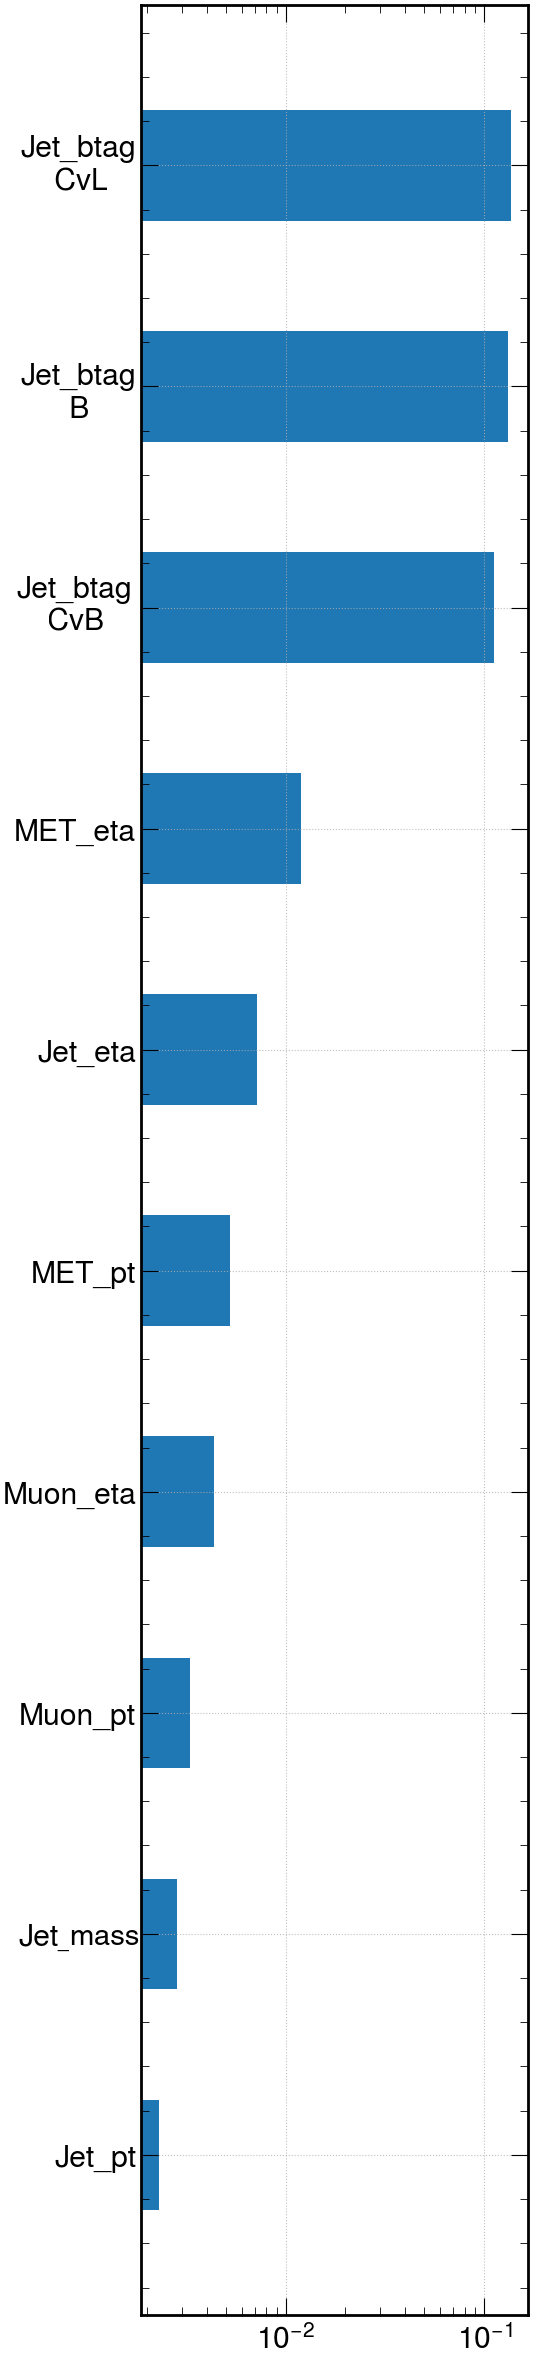
\includegraphics[height=0.92\textheight]{fig//chap08-kin_reco/ranking1D.png}
        \captionof{figure}{Unidimensional feature ranking using the metric $d$ between flattened signal observables and \ttbar semileptonic observables }
        \label{fig:1Drank}
\end{minipage}
\hfill
\begin{minipage}{0.62\linewidth}
\section{Unidimensional feature ranking}
The most straightforward approach for identifying discriminative features that separate the signal from the background is to examine the distributions of various observables and select those with the most distinct shapes.\\
The "shape difference" between two histograms can be quantified by the following metric
\begin{equation}
    d=\frac{1}{2}\sum_b \bigg| y_b^{(1)}-y_b^{(2)} \bigg|
\end{equation}
where $y_b^{(i)}$ is the bin height of the b-th bin of the i-th histogram. The histograms are normalized such that their integral is 1.\\
\\
The metric $d$ is computed between the signal and the $\ttbar$ semileptonic process, which is the primary source of background.\\
All observables are flattened, \ie all objects in the events are pooled together in the same histograms, neglecting the event's structure.\\
\\
The ranking is performed in the Muon channel, after the preselection.\\\\
The outcome of the unidimensional ranking is shown in \Fig{fig:1Drank} and, without any surprise, the observables with the highest ranking are the ones related to the b-tagging with $d\sim 0.1$, while Other observables yield results that are an order of magnitude smaller, and the latest are due mostly to statistical fluctuations.\\
\\
However, this method is not satisfactory since it does not account for correlations between the observables. Therefore, more sophisticated multivariate methods, such as neural networks, will be employed.\\\\\\\\\\    
\end{minipage}
\end{minipage}
\section{Event classification}
\section{Signal rate extraction}
\subsection{Systematic uncertainties}
\section{Ratio extraction}
\subsection{Systematic uncertainties}